\documentclass[]{article}
\usepackage{lmodern}
\usepackage{amssymb,amsmath}
\usepackage{ifxetex,ifluatex}
\usepackage{fixltx2e} % provides \textsubscript
\ifnum 0\ifxetex 1\fi\ifluatex 1\fi=0 % if pdftex
  \usepackage[T1]{fontenc}
  \usepackage[utf8]{inputenc}
\else % if luatex or xelatex
  \ifxetex
    \usepackage{mathspec}
  \else
    \usepackage{fontspec}
  \fi
  \defaultfontfeatures{Ligatures=TeX,Scale=MatchLowercase}
\fi
% use upquote if available, for straight quotes in verbatim environments
\IfFileExists{upquote.sty}{\usepackage{upquote}}{}
% use microtype if available
\IfFileExists{microtype.sty}{%
\usepackage{microtype}
\UseMicrotypeSet[protrusion]{basicmath} % disable protrusion for tt fonts
}{}
\usepackage[margin=1in]{geometry}
\usepackage{hyperref}
\hypersetup{unicode=true,
            pdftitle={Simulation of fixed and random effect},
            pdfauthor={Xuelong Wang},
            pdfborder={0 0 0},
            breaklinks=true}
\urlstyle{same}  % don't use monospace font for urls
\usepackage{graphicx,grffile}
\makeatletter
\def\maxwidth{\ifdim\Gin@nat@width>\linewidth\linewidth\else\Gin@nat@width\fi}
\def\maxheight{\ifdim\Gin@nat@height>\textheight\textheight\else\Gin@nat@height\fi}
\makeatother
% Scale images if necessary, so that they will not overflow the page
% margins by default, and it is still possible to overwrite the defaults
% using explicit options in \includegraphics[width, height, ...]{}
\setkeys{Gin}{width=\maxwidth,height=\maxheight,keepaspectratio}
\IfFileExists{parskip.sty}{%
\usepackage{parskip}
}{% else
\setlength{\parindent}{0pt}
\setlength{\parskip}{6pt plus 2pt minus 1pt}
}
\setlength{\emergencystretch}{3em}  % prevent overfull lines
\providecommand{\tightlist}{%
  \setlength{\itemsep}{0pt}\setlength{\parskip}{0pt}}
\setcounter{secnumdepth}{5}
% Redefines (sub)paragraphs to behave more like sections
\ifx\paragraph\undefined\else
\let\oldparagraph\paragraph
\renewcommand{\paragraph}[1]{\oldparagraph{#1}\mbox{}}
\fi
\ifx\subparagraph\undefined\else
\let\oldsubparagraph\subparagraph
\renewcommand{\subparagraph}[1]{\oldsubparagraph{#1}\mbox{}}
\fi

%%% Use protect on footnotes to avoid problems with footnotes in titles
\let\rmarkdownfootnote\footnote%
\def\footnote{\protect\rmarkdownfootnote}

%%% Change title format to be more compact
\usepackage{titling}

% Create subtitle command for use in maketitle
\newcommand{\subtitle}[1]{
  \posttitle{
    \begin{center}\large#1\end{center}
    }
}

\setlength{\droptitle}{-2em}

  \title{Simulation of fixed and random effect}
    \pretitle{\vspace{\droptitle}\centering\huge}
  \posttitle{\par}
    \author{Xuelong Wang}
    \preauthor{\centering\large\emph}
  \postauthor{\par}
      \predate{\centering\large\emph}
  \postdate{\par}
    \date{2018-08-03}

\usepackage{float,amsmath, bbm, siunitx, bm}
\floatplacement{figure}{H}
\newcommand{\indep}{\rotatebox[origin=c]{90}{$\models$}}

\begin{document}
\maketitle

{
\setcounter{tocdepth}{2}
\tableofcontents
}
\section{Motivation}\label{motivation}

Based on the previous simulations results, we found that the proposed
method is able to work well on estimating the interactive effect in
certain situation. However, because of the interaction terms the
covariates cannot be \textbf{Independent} anymore. Thus, we may need to
conduct a series simulations with different setup in order to get a
large picture of what situation the proposed method can work well.

\section{Background}\label{background}

\subsection{GCTA method and proposed
method}\label{gcta-method-and-proposed-method}

In the GCTA method, the author suggests that the causal covariates
should be independent themselves and also be independent with non-causal
covariates. Therefore, to ensure the GCTA method is able to work
appropriately, we need to make sure the independence among the
covariates.

The approach of the proposed method is to uncorrelated the observed
covariates by using a linear transformation, i.e. \(Z = XA^{-1}\). Given
\(X \sim N(0, \Sigma)\), we can using the proposed method to get a
independent covariates. Thus, this method should work well when X's
columns are correlated to each other, which is also supported by
simulation results on the main effects with normal correlated
distributions.

How to reduce the correlation (the linear transformation) is important
part of the proposed method. Because we want to the decorrelated the
covariates so that they become independent. We don't want to pick up to
much noise during the decorrelation procedure. This is not the main
topic of this simulation, but we will do a more details study on the
decorrelation.

\subsection{Adding the interactive
terms}\label{adding-the-interactive-terms}

From the model point of view, it actually doesn't change a lot. We can
consider the interactive term as another part of covariates. However,
since the interactive effects have a strong relation with main effect,
that causes the estimation of variance of interactive effect
complicated.

\subsubsection{Issues}\label{issues}

\begin{align*}
Var(Y_i) &= Var(X_i^T\beta + X_i^T\Gamma X_i) + Var(\epsilon_i) \\
         &= Var(X_i^T\beta) + Var(X_i^T\Gamma X_i) + 2Cov(X_i^T\beta, X_i^T\Gamma X_i) + Var(\epsilon_i) \\
\end{align*}

\begin{enumerate}
\def\labelenumi{\arabic{enumi}.}
\tightlist
\item
  There is an additional terms \(Cov(X_i^T\beta, X_i^T\Gamma X_i)\)
\item
  The main effect \(X_i\) and \(X_i X_j\) are not independent and cannot
  be independent anymore
\item
  In order to keep the variance structure, we can only apply the linear
  transformation on the main effects, not the interactive effects.
\end{enumerate}

\subsubsection{Solutions}\label{solutions}

For the first issue, there are basic two different approach.

\begin{enumerate}
\def\labelenumi{\arabic{enumi}.}
\item
  If X or after some transformation follows normal distributions, then
  the \(Cov(X_i^T\beta, X_i^T\Gamma X_i)\) will be zero. More
  specifically, as long as the 3rd moments are 0 the correlation of main
  and interactive effect should be zero.
\item
  If we assume \(\beta's\) or \(\Gamma's\) are independent random
  variables, then the correlation should also be round zero.
\end{enumerate}

For the second issue, the simulation studies shows that the the proposed
method can work well under the normal distribution setup. So it suggests
that the Independence assumption may not be that restricted, at least
under the Normal distribution. One guess is that under normal
distribution the covariates of main and interactive is zero
\(Cov(X_i^T\beta, X_i^T\Gamma X_i) = 0\), which means they are
un-correlated. Although un-correlation can not guarantee independence,
it shows non-linear relation between main and interactive effects.

Thus, the main idea is to first transform the covariates into
normal-like distribution and applied the proposed method.

\section{Simulation}\label{simulation}

To get a better and larger picture of how well the proposed method's
estimations, we conduct a series simulation with different setup.

The main factors are

\begin{enumerate}
\def\labelenumi{\arabic{enumi}.}
\tightlist
\item
  Distribution of X\\
\item
  Independence and Dependence of X\\
\item
  Fixed or Random of main effect \(\beta's\)\\
\item
  Fixed or Random of interaction effect \(\Gamma's\)
\end{enumerate}

\subsection{Simulation procedure}\label{simulation-procedure}

\begin{figure}
\centering
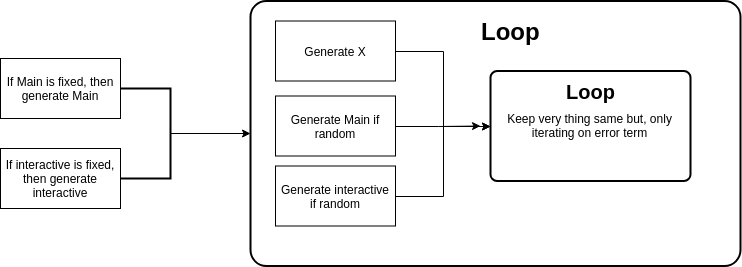
\includegraphics{./simulation_workflow.png}
\caption{Simulation workflow}
\end{figure}

\section{X follows Normal
distributions}\label{x-follows-normal-distributions}

If we can assume that X has normal distribution then the problem become
more straightforward, because the correlation of main and interactive
effects are zero. Besides, we don't need to transform X in order to make
it looks like a normal distribution.

\subsection{Independent}\label{independent}

Based on the previous simulation (from the Proposal), if X is normal and
independent, then both proposed and original GCTA method can estimate
the main and interaction effects well. This is indirectly suggest that
the dependence between main and interactive may not be a big issue.

\subsection{Dependent (correlated)}\label{dependent-correlated}

If the X's are normal but correlated with each other, then it's not easy
to estimate the interactive correctly. Based on previous simulation's
results, the proposed method can work much better than the original GCTA
when \(\beta\), the main effect, is fixed. However when the main
coefficients are not fixed then there is a big bias for the interaction
estimation of proposed method. A guess is that if the \(\beta\) is not
linear transformation of may affect the \(Var(X_i^T\Gamma X_i)\).

\subsubsection{\texorpdfstring{\(\beta\) is fixed and \(\Gamma\) is
fixed}{\textbackslash{}beta is fixed and \textbackslash{}Gamma is fixed}}\label{beta-is-fixed-and-gamma-is-fixed}

The estimation and true values

\[
    Var(X_i^T\beta) = \beta^T \Sigma \beta
\]

\begin{align*}
    Var(X_i^T\Gamma X_i) = 2tr(\Gamma \Sigma \Gamma \Sigma) + 0
\end{align*}

Simulation result

\begin{figure}
\centering
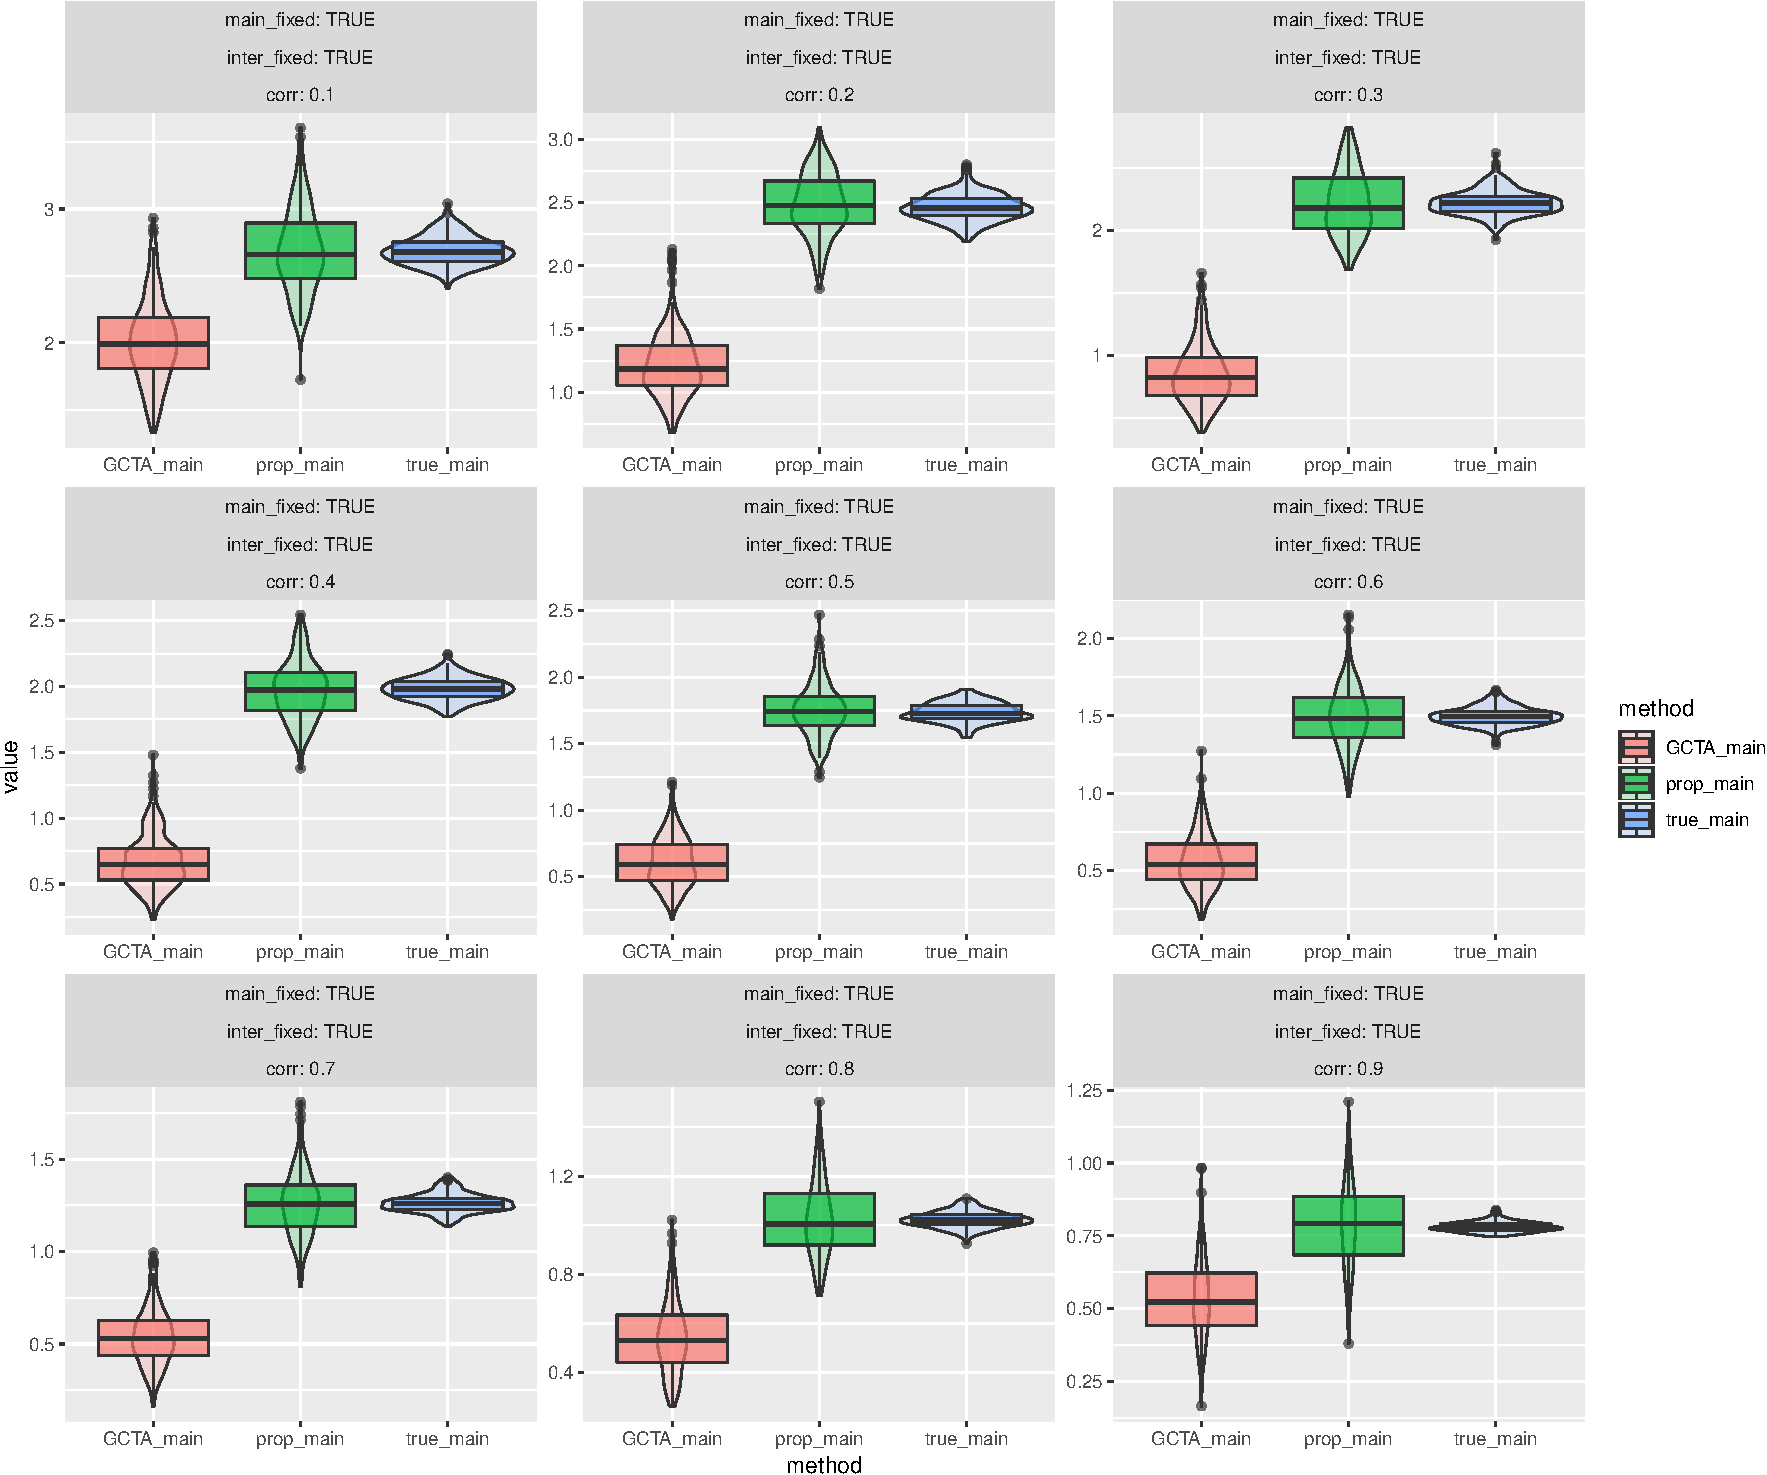
\includegraphics{Simulation_report_files/figure-latex/main_fixed_fixed_normal-1.pdf}
\caption{main effect of normal fixed main and interaction}
\end{figure}

\begin{figure}
\centering
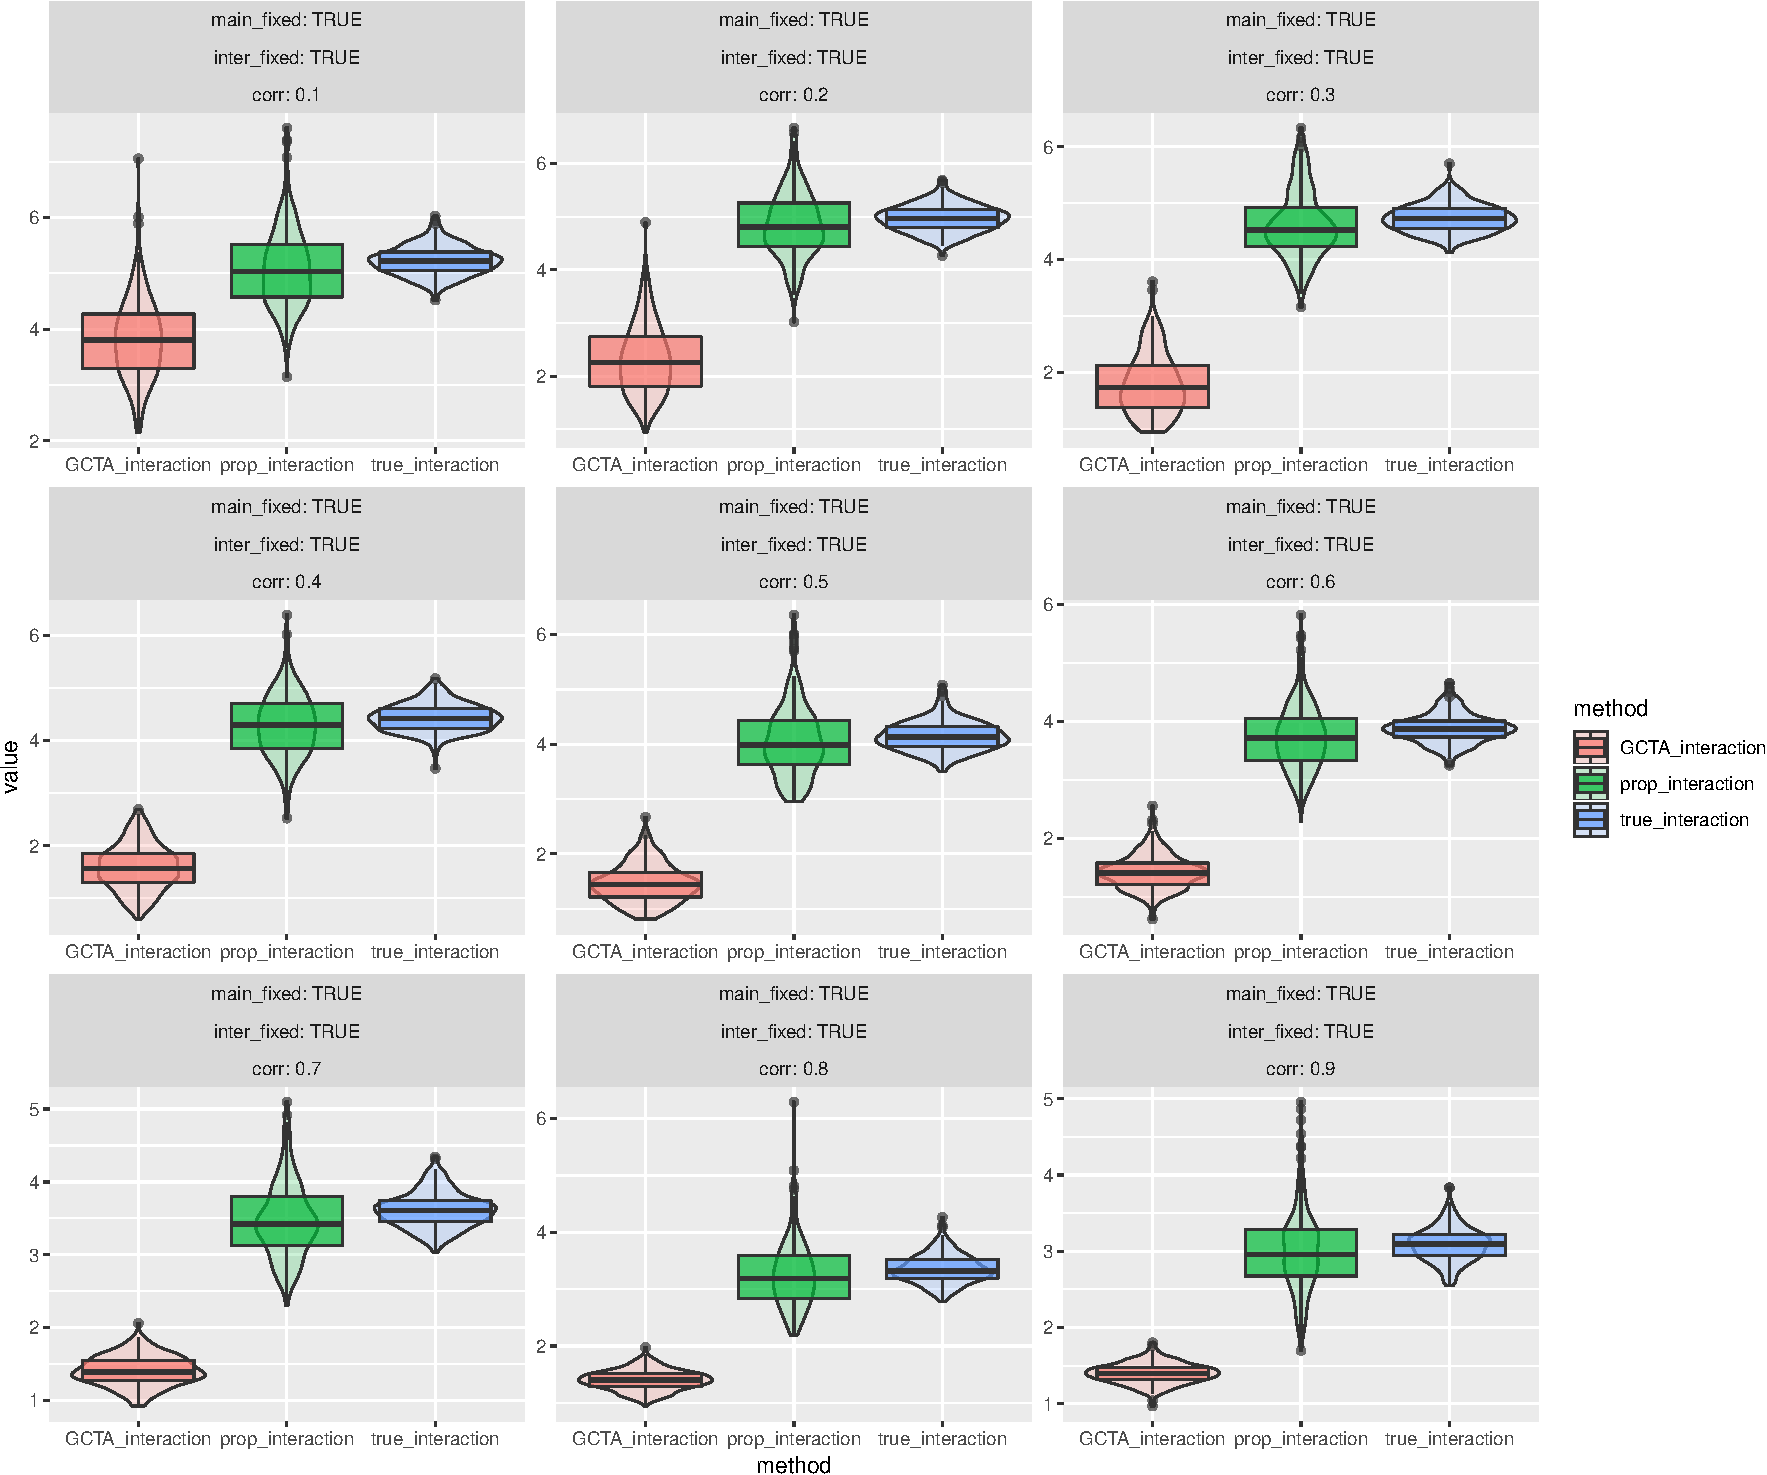
\includegraphics{Simulation_report_files/figure-latex/inter_fixed_fixed_normal-1.pdf}
\caption{interactive effect of normal fixed main and interaction}
\end{figure}

\clearpage

\subsubsection{\texorpdfstring{\(\beta\) is fixed and \(\Gamma\) is
random}{\textbackslash{}beta is fixed and \textbackslash{}Gamma is random}}\label{beta-is-fixed-and-gamma-is-random}

\[
    Var(X_i^T\beta) = \beta^T \Sigma \beta
\]

\begin{align*}
    Var(X_i^T\Gamma X_i) &= E(Var(X_i^T\Gamma X_i|X_i = x_i)) + Var(E(X_i^T\Gamma X_i|X_i = x_i)) \\ 
                         &= E(Var(X_i^T\Gamma X_i|X_i = x_i))
\end{align*}

Simulation result

\begin{figure}
\centering
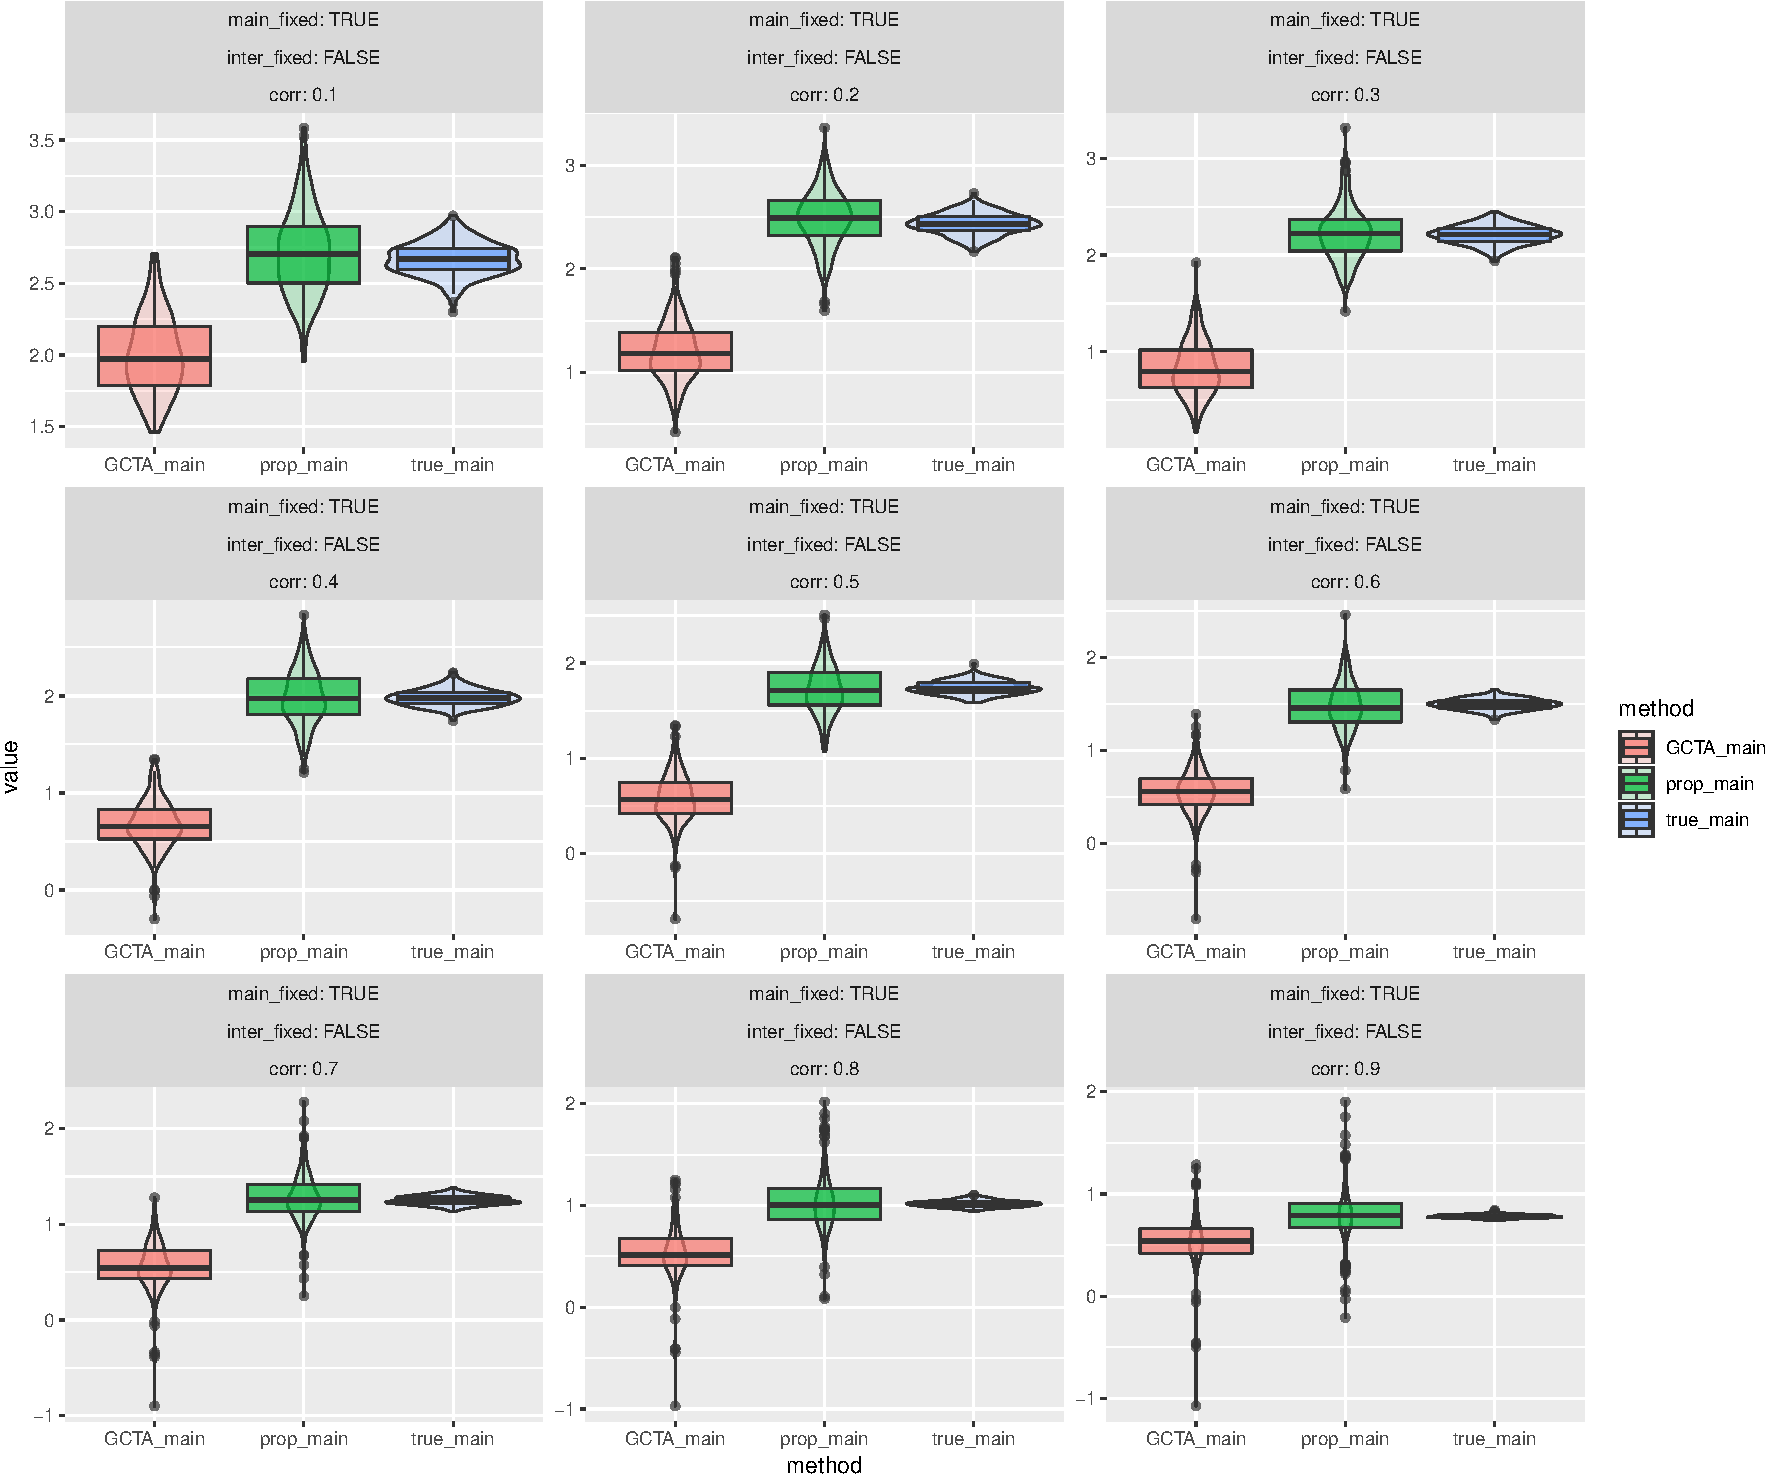
\includegraphics{Simulation_report_files/figure-latex/main_fixed_random_normal-1.pdf}
\caption{main effect of normal fixed main and random interaction}
\end{figure}

\begin{figure}
\centering
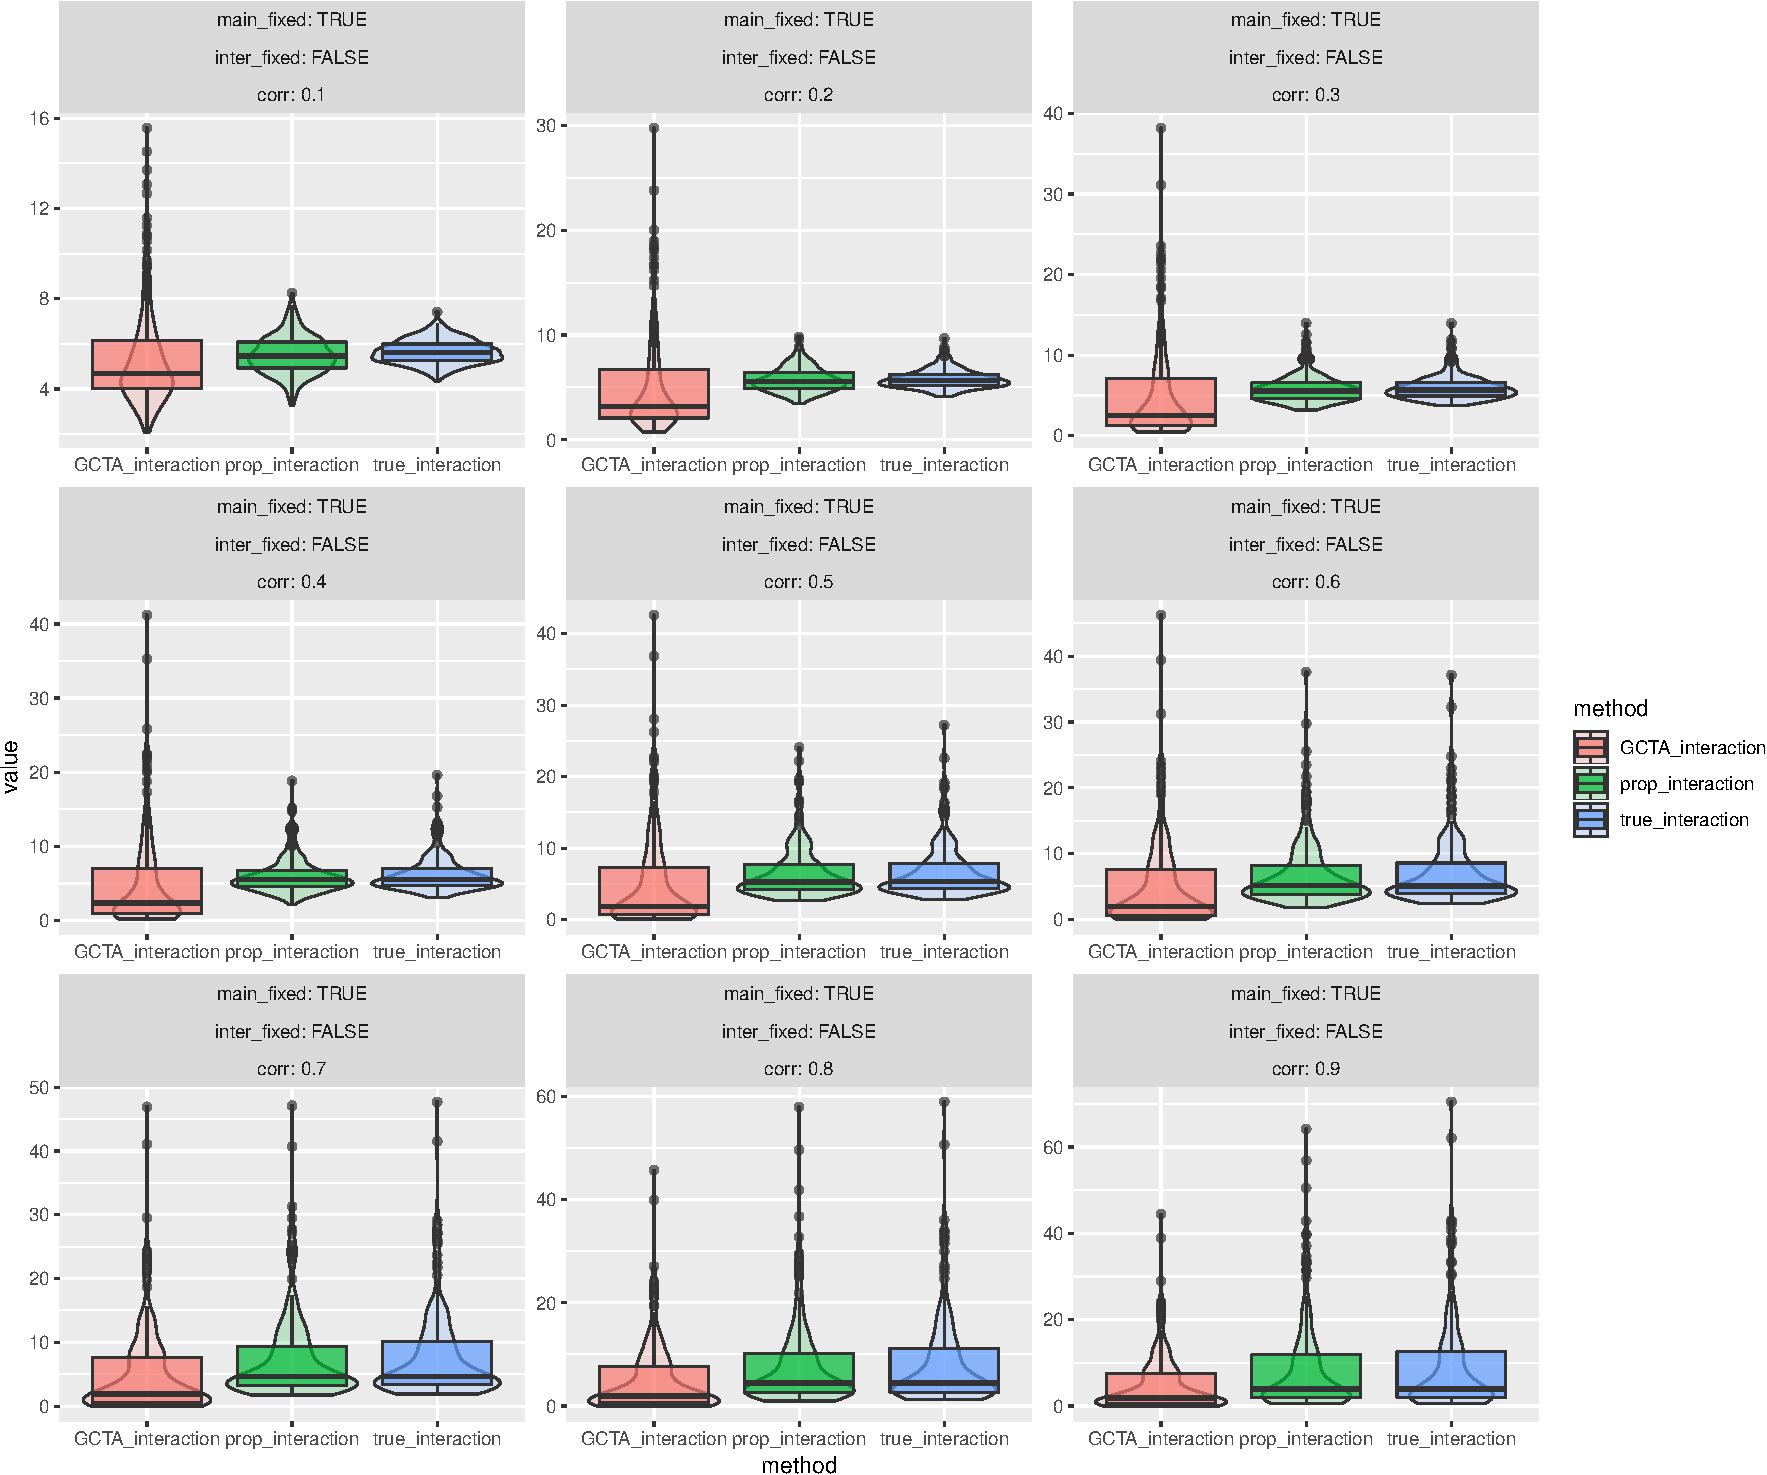
\includegraphics{Simulation_report_files/figure-latex/inter_fixed_random_normal-1.pdf}
\caption{interactive effect of normal fixed main and random interaction}
\end{figure}

\clearpage

\subsubsection{\texorpdfstring{\(\beta\) is random and \(\Gamma\) is
random}{\textbackslash{}beta is random and \textbackslash{}Gamma is random}}\label{beta-is-random-and-gamma-is-random}

\begin{align*}
    Var(X_i^T\beta) &= E(Var(X_i^T\beta|X_i = x_i)) + Var(E(X_i^T\beta|X_i = x_i))\\
                    &= E(Var(X_i^T\beta|X_i = x_i)) + 0 \\
                    &= E(X_i^T \Sigma_{\beta} X_i)  \tag*{If $\Sigma_{\beta} = I_p$}\\
                    &= E(X_i^TX_i)
\end{align*}

\begin{align*}
    Var(X_i^T\Gamma X_i) &= E(Var(X_i^T\Gamma X_i|X_i = x_i)) + Var(E(X_i^T\Gamma X_i|X_i = x_i)) \\ 
                         &= E(Var(X_i^T\Gamma X_i|X_i = x_i))
\end{align*}

\begin{figure}
\centering
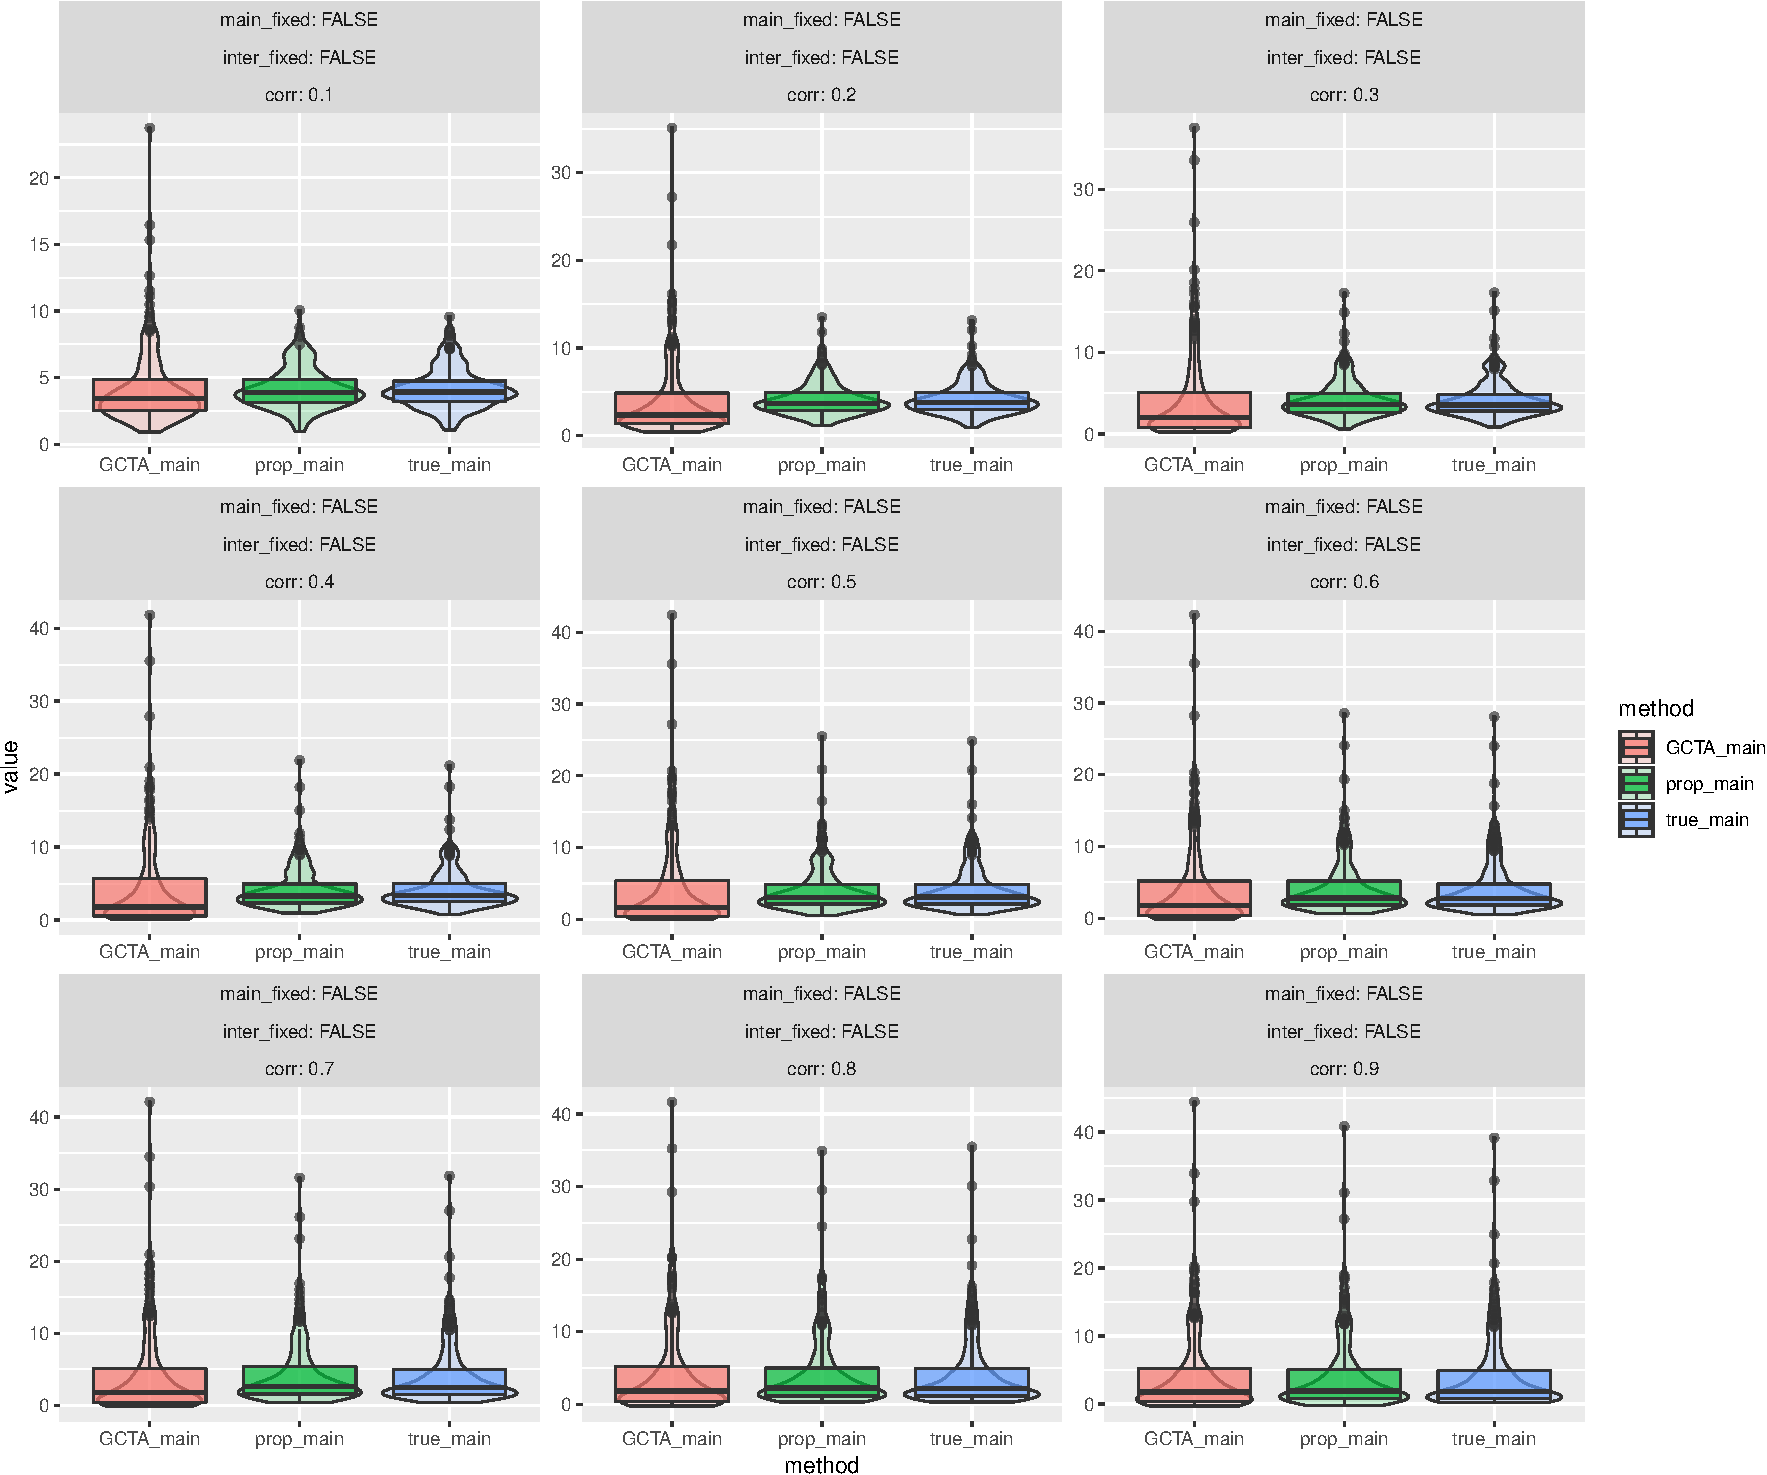
\includegraphics{Simulation_report_files/figure-latex/main_random_random_normal-1.pdf}
\caption{main effect of normal random main and interaction}
\end{figure}

\begin{figure}
\centering
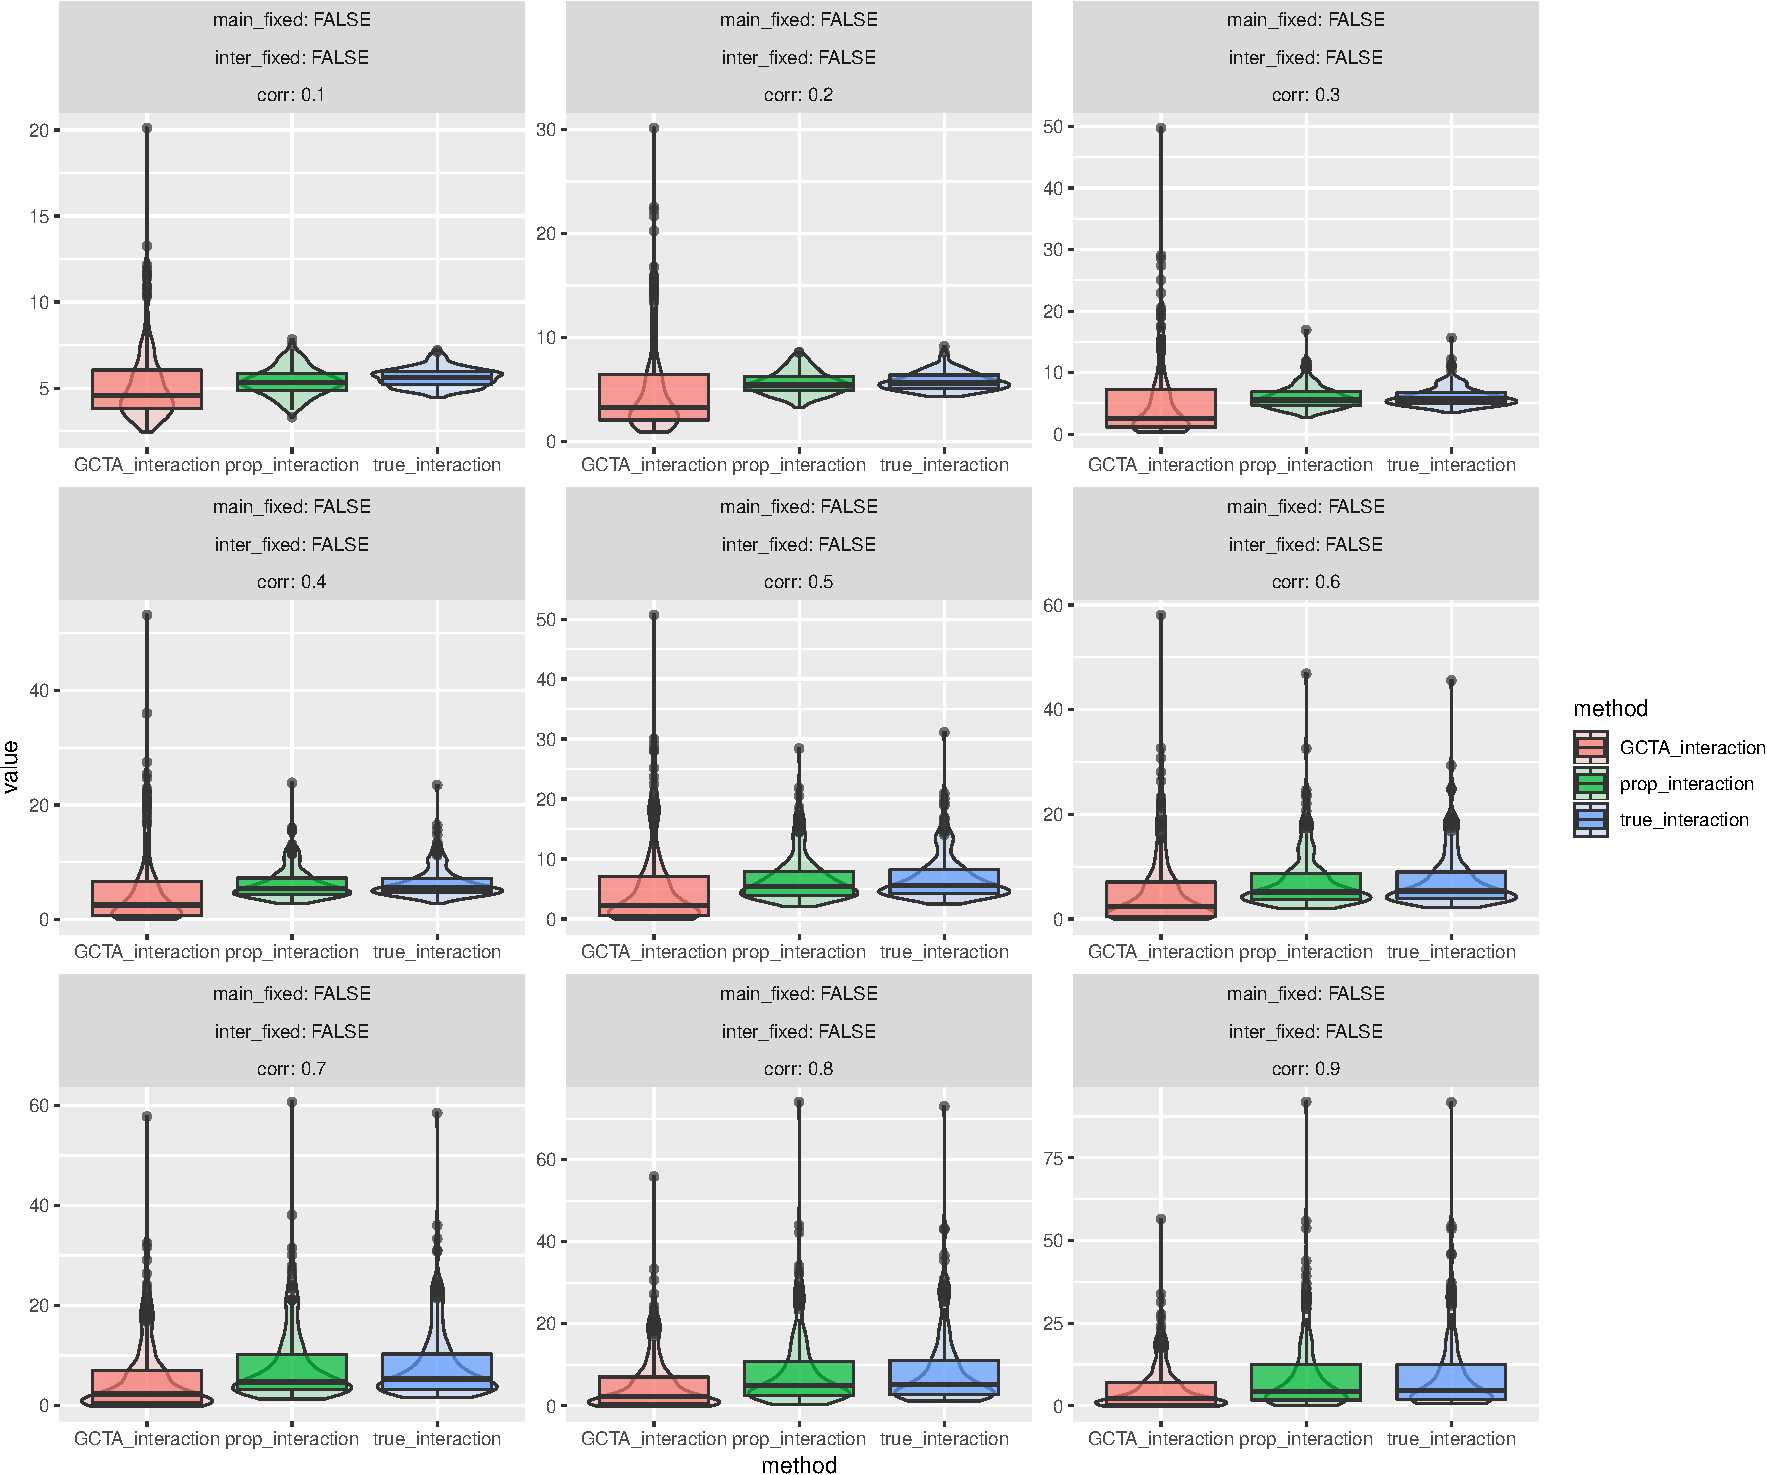
\includegraphics{Simulation_report_files/figure-latex/inter_random_random_normal-1.pdf}
\caption{interactive effect of normal random main and interaction}
\end{figure}

\section{Conclusion}\label{conclusion}

\section{Further work}\label{further-work}


\end{document}
